% \begin{figure}[!t]
%   \centering
%   \vspace{-5pt}
%   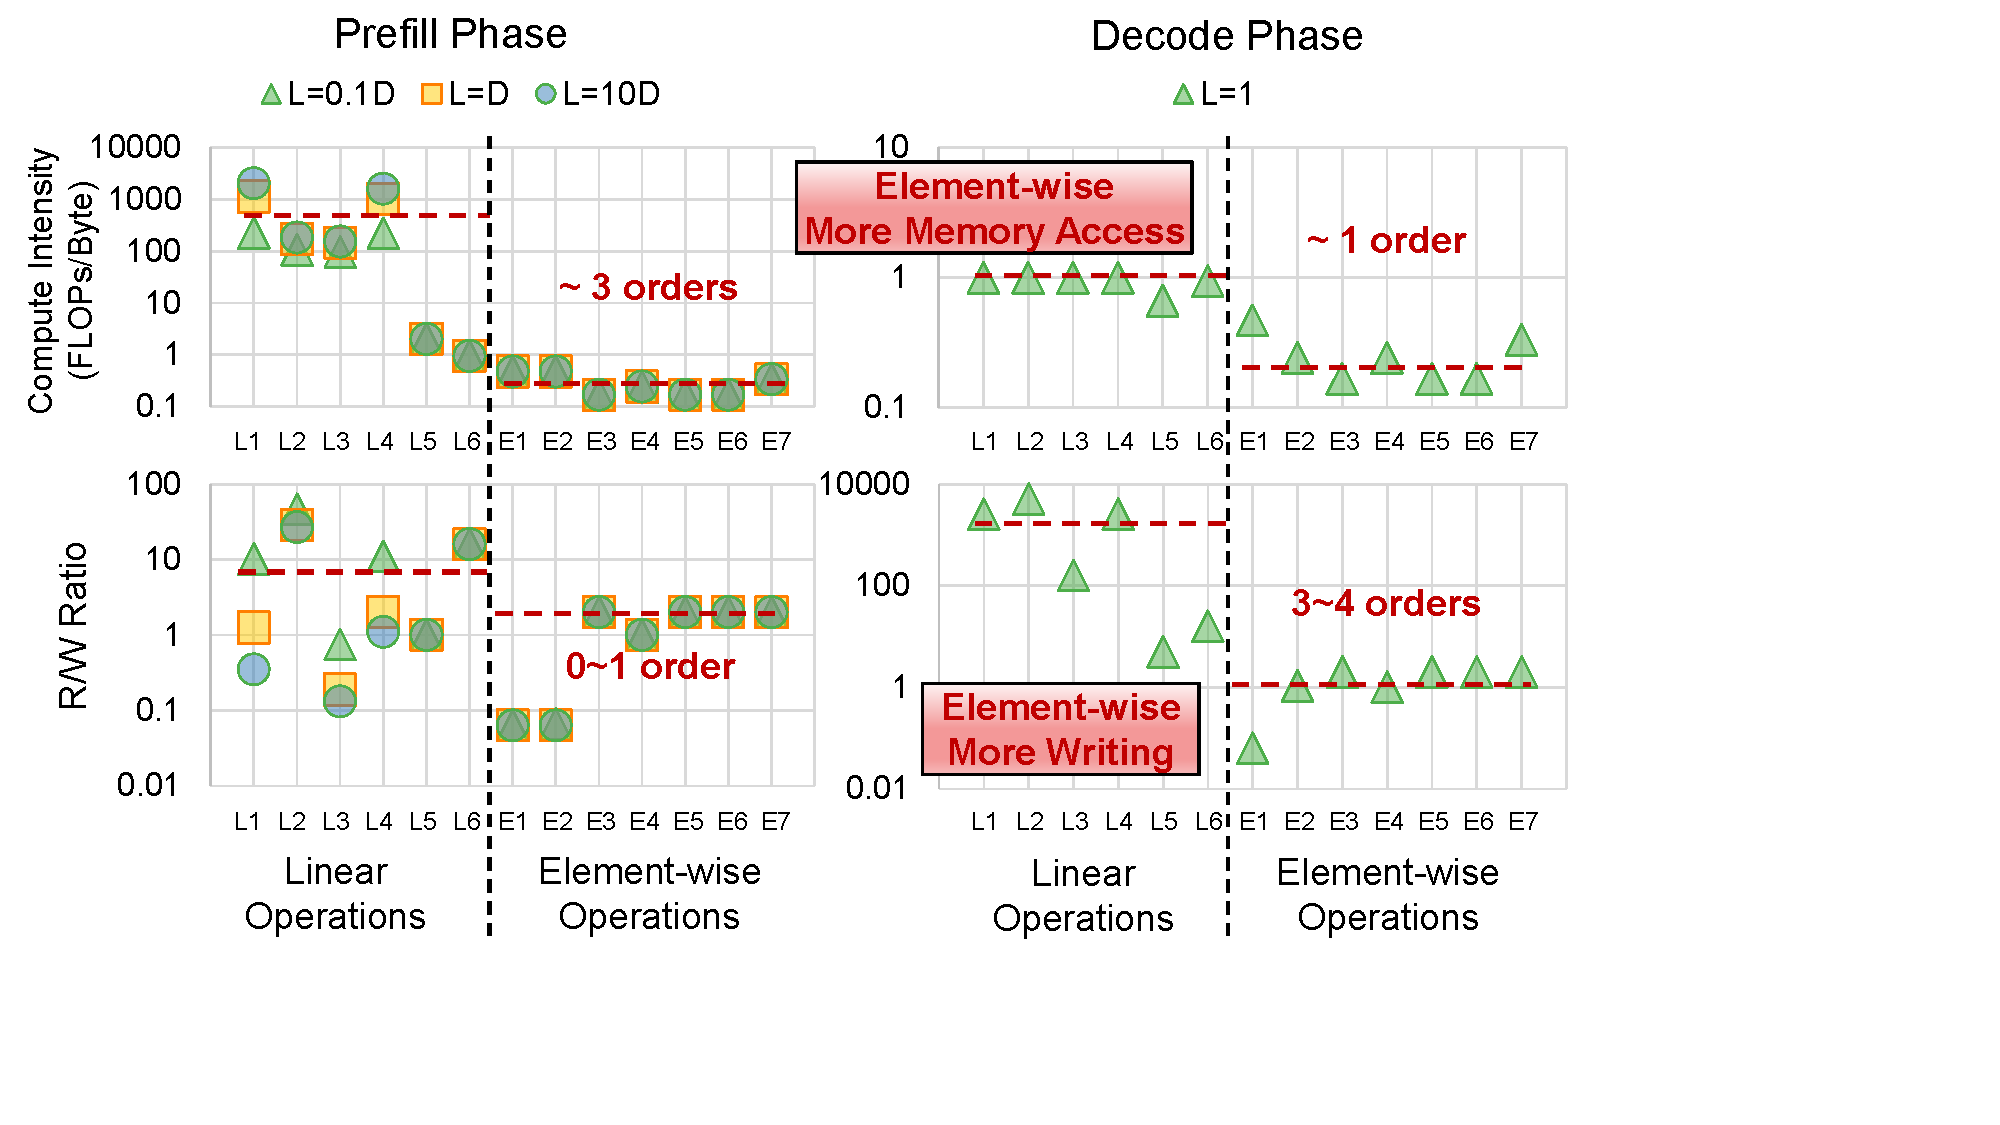
\includegraphics[width=0.48\textwidth]{figures/method2/m2_challenge.pdf}
%   \vspace{-20pt}
%   \caption{The difference of compute intensity and read/write ratio with different sequence length input in Mamba. Compared with linear operations, element-wise operations need more memory access and more memory writing.}
%   \vspace{-20pt}
%   \label{fig:read-write-ratio}
% \end{figure}

% \section{Intra-/Inter-Operation Buffer Management Strategy}\label{sec:method2}

% \subsection{Challenge}
% Linear and element-wise operations are two dominant operations in Mamba processing.
% The feature of memory access for these two kinds shows three typical paradigms, that is, reading $2\times2N$ data and writing $2\times2$, $2N$, and $2N^{2}$ corresponding to linear projection (Linear), element-wise addition or multiplication (Element-wise 1), and element-wise outer product (Element-wise 2), as shown in Figure~\ref{fig:overview} right bottom. 
% As shown in Figure~\ref{fig:read-write-ratio}, we depict a detailed breakdown of the memory read/write ratio with different input sequence length for various operations during Mamba computation process. 
% It shows that the read/write ratio of the three operations differs by more than three orders of magnitude.
% For linear operations with more input and less output, existing optimization methods primarily focus on tiling~\cite{li2019coordinated} and load the tiled input to on-chip buffer to maximize data sharing.
% However, due to the computational characteristic of element-wise operations with more output and less input, it is redundant to apply input sharing methods like tiling.

% \subsection{Motivation and Insights}
% The computational characteristics of linear operations require reduction and input sharing, leading to a higher read/write ratio, which is suitable for existing input data sharing methods during each operation processing.
% By reviewing Figure~\ref{fig:mamba_block}, we find that the element-wise operations are closely spaced within the SSM computation process.
% And during the SSM process, the outputs of element-wise operations such as $\Delta A$, $\Delta B$, and $h$ are accessed repeatedly. 
% Storing these output of element-wise operations on the on-chip buffer can significantly reduce the overhead of memory access for the next operation.
% Therefore, our key insight is to \textbf{adjust different buffer management strategies for different operation types to maximize the data sharing with intra-operation and inter-operation.}

% \begin{figure}[!t]
%   \centering
%   \vspace{-5pt}
%   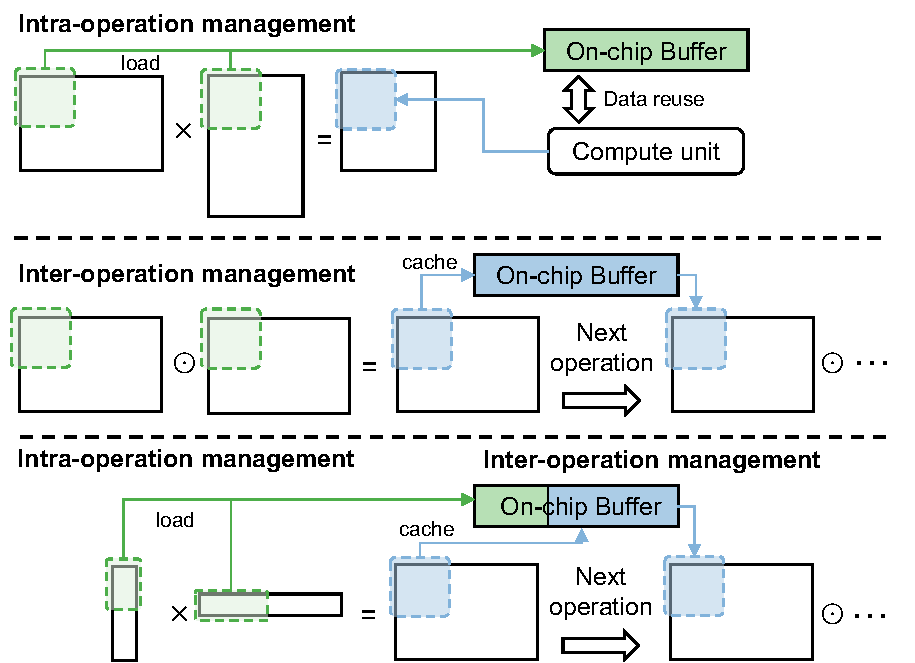
\includegraphics[width=0.48\textwidth]{figures/method2/buffer_management.pdf}
%   \vspace{-20pt}
%   \caption{MARCA buffer management strategy for different operations.}
%   \vspace{-20pt}
%   \label{fig:buffer_management}
% \end{figure}

% \subsection{Approach}

% Our operation-wise buffer management (BM) strategies contain intra-operation and inter-operation methods as shown in Figure ~\ref{fig:buffer_management}. 
% Intra-operation buffer management (Intra-BM) is used to discover and manage data sharing within individual operations, while inter-operation buffer management (Inter-BM) is used to discover and manage data sharing between operations.

% \textbf{Intra-operation Management.}
% For linear operations, the whole on-chip buffers are configured as read buffers. The memory access handler loads linear inputs from global memory to fill the buffer. The computing unit then sequentially reads the required data from the buffer, performs calculations, and writes the computed results back to global memory.
% For element-wise 2 operation, even though the read/write ratio is relatively low, it can be effectively regarded as a matrix multiplication with two reduction dimensions of size 1, hence requiring data sharing among inputs. Therefore, we reserve a small fraction region of the on-chip buffer to store them.
% % two input $I$ and $J$ can share with each other, because $I_{00}$ need to compute with $J_{00}$, $J_{01}$, $J_{02}$, and $J_{03}$. Therefore, we reserve a small fraction region of the buffer pool to store these two input.

% \textbf{Inter-operation Management.}
% For element-wise 1, there is no data reuse in the computation of input data. 
% The basic approach involves reading from global memory and directly writing back after computation. For individual computations, data reuse optimization like tiling is not feasible.
% For element-wise 1 and 2 operations, to maximize buffer utilization, we primarily optimize data sharing among adjacent element-wise operations. 
% As shown in equation~\ref{eq:ssm}, the update of hidden state $h$ is obtained by adding the product of $\Delta A$ and $h$ with the product of $\Delta B$ and $x$. Therefore, during the continuous updating process of state $h$, $h$ needs to be read and written $L$ times repeatedly. Additionally, the corresponding $\Delta A$, $\Delta B$, and $x$ need to be read $L$ times repeatedly. Hence, for element-wise operations concentrated in the SSM process, we cache the above immediate result in the buffer.

% Through an operation-wise buffer management strategy, our method maximizes the reduction in memory access and minimizes idle computational resources, thereby accelerating the Mamba computation process.

